\documentclass[aspectratio=169,11pt]{beamer}
\usepackage{amsmath,amssymb}
\usepackage{booktabs}
\usepackage{graphicx}
\usepackage{tikz}
\usepackage[T1]{fontenc}
\usepackage{lmodern}
\definecolor{courseblue}{RGB}{0,91,155}
\definecolor{courseorange}{RGB}{190,72,20}
\setbeamercolor{structure}{fg=courseblue}
\setbeamercolor{frametitle}{fg=courseblue}
\setbeamercolor{alerted text}{fg=courseorange}
\setbeamertemplate{navigation symbols}{}
\setbeamertemplate{footline}[frame number]
\setbeamertemplate{itemize items}[circle]
\title{Elliptical slice sampling}
\subtitle{A two-variable example and MATLAB implementation}
\author{Econometrics 32706}
\date{}

\begin{document}
\begin{frame}
  \titlepage
\end{frame}

\begin{frame}{The target distribution}
  Suppose a latent vector has a Gaussian prior and a likelihood:
  \[
    f\sim\mathcal N(0,K),
    \qquad
    p(f\mid y)\ \propto\ \mathcal N(f;0,K)L(f).
  \]
  \begin{itemize}
    \item Elliptical slice sampling (ESS) updates the whole vector \(f\).
    \item We need a draw from \(\mathcal N(0,K)\) and a function that returns
          \(\log L(f)\).
    \item The likelihood can be non-Gaussian. The prior covariance \(K\) is
          held fixed during this update.
  \end{itemize}
\end{frame}

\begin{frame}{A proposal on a Gaussian ellipse}
  From the current state \(f\), draw an independent
  \(\nu\sim\mathcal N(0,K)\). For any angle \(\theta\), define
  \[
    f(\theta)=f\cos\theta+\nu\sin\theta.
  \]
  \begin{center}
    \begin{tabular}{@{}ccl@{}}
      \toprule
      Angle & Candidate & Meaning\\
      \midrule
      \(0\) & \(f\) & current state\\
      \(\pi/2\) & \(\nu\) & independent prior draw\\
      \(\pi\) & \(-f\) & opposite point on the ellipse\\
      \bottomrule
    \end{tabular}
  \end{center}
  Rotating the pair \((f,\nu)\) preserves their joint Gaussian prior.
  The likelihood determines which angles are eligible.
\end{frame}

\begin{frame}{Why the rotation preserves the Gaussian prior}
  Under the prior, \(f\) and \(\nu\) are independent draws from
  \(\mathcal N(0,K)\). Rotate \emph{both} vectors:
  \[
    \begin{aligned}
      f_\theta   &= f\cos\theta+\nu\sin\theta,\\
      \nu_\theta &= -f\sin\theta+\nu\cos\theta.
    \end{aligned}
  \]
  The new first vector still has covariance \(K\):
  \[
    \operatorname{Var}(f_\theta)
      =(\cos^2\theta+\sin^2\theta)K=K,
    \qquad
    \operatorname{Cov}(f_\theta,\nu_\theta)=0.
  \]
  The rotated pair therefore has the same joint Gaussian prior.
  In ESS, the likelihood slice then selects an eligible angle, bringing
  the observed data into the update.
\end{frame}

\begin{frame}{What orthogonal means here}
  The coefficients in the two rotation equations form the matrix
  \[
    R(\theta)=
    \begin{pmatrix}
      \cos\theta & \sin\theta\\
      -\sin\theta & \cos\theta
    \end{pmatrix},
    \qquad R(\theta)^\top R(\theta)=I.
  \]
  Its columns have length one and are perpendicular. Therefore, mixing
  the pair \((f,\nu)\) does not change its combined squared length:
  \[
    \|f_\theta\|^2+\|\nu_\theta\|^2
      =\|f\|^2+\|\nu\|^2.
  \]
  At \(\theta=\pi/2\), the pair becomes
  \((f_\theta,\nu_\theta)=(\nu,-f)\): the vectors swap roles,
  with one sign changed.
\end{frame}

\begin{frame}{One ESS update}
  \begin{enumerate}
    \setlength{\itemsep}{0.55em}
    \item Draw \(\nu\sim\mathcal N(0,K)\) and \(u\sim U(0,1)\). Set the
      log slice level \(\ell_\star=\log L(f)+\log u\).
    \item Draw an initial angle \(\theta\sim U(0,2\pi)\).
      Set \([\theta_{\min},\theta_{\max}]=[\theta-2\pi,\theta]\).
    \item Test \(f(\theta)=f\cos\theta+\nu\sin\theta\).
      If \(\log L(f(\theta))>\ell_\star\), return \(f(\theta)\).
    \item On rejection, set \(\theta_{\min}=\theta\) if \(\theta<0\);
      otherwise set \(\theta_{\max}=\theta\).
      Draw another \(\theta\) uniformly from the remaining bracket
      and return to step 3.
  \end{enumerate}
  \vspace{0.45em}
  Keep the same \(\nu\) and \(\ell_\star\) throughout this update.
\end{frame}

\begin{frame}{The initial bracket contains zero}
  The ellipse repeats every \(2\pi\):
  \[
    f(\theta)=f\cos\theta+\nu\sin\theta,
    \qquad f(2\pi k)=f\quad(k\in\mathbb Z).
  \]
  For an initial draw \(0<\theta<2\pi\), set
  \[
    \theta_{\min}=\theta-2\pi,
    \qquad
    \theta_{\max}=\theta.
  \]
  Thus \(\theta_{\min}<0<\theta_{\max}\), and the bracket
  spans exactly one full turn.
  \vspace{0.35em}
  \begin{center}
  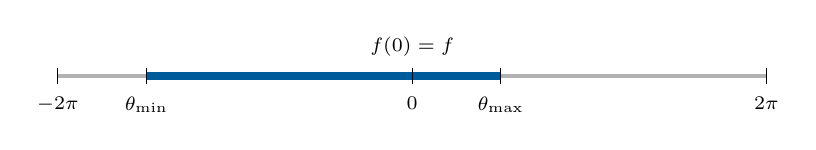
\begin{tikzpicture}[x=0.9cm,y=0.7cm,
                      every node/.style={font=\scriptsize}]
    \draw[line width=1.3pt,gray!60] (1,0)--(11,0);
    \draw[line width=3pt,courseblue] (2.25,0)--(7.25,0);
    \foreach \x in {1,2.25,6,7.25,11}
      \draw[black] (\x,-0.15)--(\x,0.15);
    \node[below] at (1,-0.2) {\(-2\pi\)};
    \node[below] at (2.25,-0.2) {\(\theta_{\min}\)};
    \node[below] at (6,-0.2) {\(0\)};
    \node[below] at (7.25,-0.2) {\(\theta_{\max}\)};
    \node[below] at (11,-0.2) {\(2\pi\)};
    \node[above] at (6,0.18) {\(f(0)=f\)};
  \end{tikzpicture}
  \end{center}
\end{frame}

\begin{frame}{Why the initial endpoints agree}
  At initialization, \(\theta_{\min}=\theta_{\max}-2\pi\).
  Periodicity gives
  \[
    \begin{aligned}
      f(\theta_{\min})
        &=f\cos(\theta_{\max}-2\pi)
          +\nu\sin(\theta_{\max}-2\pi)\\
        &=f\cos\theta_{\max}+\nu\sin\theta_{\max}
         =f(\theta_{\max}).
    \end{aligned}
  \]
  This equality holds for every \(f\), \(\nu\), and initial angle.
  It says that the endpoints are the \emph{same point} on the ellipse;
  it does not say that the point is \(\nu\) or \(f\).
  \vspace{0.6em}

  Separately, \(f(0)=f\). Keeping \(0\) in the bracket preserves
  a known acceptable angle while the sampler searches.
\end{frame}

\begin{frame}{The drawn angle sets both endpoints}
  At initialization, draw \(\theta\in(0,2\pi)\) and set
  \[
    [\theta_{\min},\theta_{\max}]=[\theta-2\pi,\theta].
  \]
  These two draws give different brackets and endpoint values:
  \begin{center}
    \renewcommand{\arraystretch}{1.55}
    \begin{tabular}{@{}ccc@{}}
      \toprule
      Drawn \(\theta\) & Bracket \([\theta_{\min},\theta_{\max}]\)
        & Value at both endpoints\\
      \midrule
      \(\pi/2\) & \([-3\pi/2,\,\pi/2]\) & \(\nu\)\\
      \(\pi/3\) & \([-5\pi/3,\,\pi/3]\)
        & \(\tfrac12 f+\tfrac{\sqrt3}{2}\nu\)\\
      \bottomrule
    \end{tabular}
  \end{center}
  The endpoints agree because they are \(2\pi\) apart.
  Their shared value depends on the drawn angle.
  The current state \(f\) is at angle \(0\) in both brackets.
\end{frame}

\begin{frame}{Why shrinking leaves acceptable angles}
  Write \(g(\theta)=\log L(f(\theta))\).
  Since \(u\in(0,1)\), the slice level is strictly below the value at zero:
  \[
    \ell_\star=g(0)+\log u<g(0).
  \]
  If \(g\) is continuous at zero, some \(\varepsilon>0\) satisfies
  \[
    |\theta|<\varepsilon
      \quad\Longrightarrow\quad g(\theta)>\ell_\star.
  \]
  Thus a small interval around zero is acceptable.
  A rejected angle lies outside it. Shrinking the endpoint on that
  angle's side of zero keeps an acceptable interval in the bracket.
  \vspace{0.25em}
  \begin{center}
  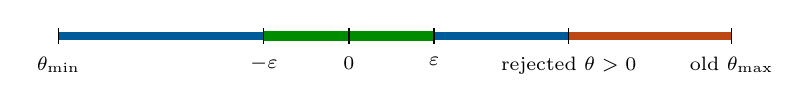
\begin{tikzpicture}[x=0.9cm,y=0.7cm,
                      every node/.style={font=\scriptsize}]
    \draw[line width=2.6pt,courseblue] (1.3,0)--(8.5,0);
    \draw[line width=2.6pt,courseorange] (8.5,0)--(10.8,0);
    \draw[line width=3.5pt,green!55!black] (4.2,0)--(6.6,0);
    \foreach \x in {1.3,4.2,5.4,6.6,8.5,10.8}
      \draw[black] (\x,-0.14)--(\x,0.14);
    \node[below] at (1.3,-0.2) {\(\theta_{\min}\)};
    \node[below] at (4.2,-0.2) {\(-\varepsilon\)};
    \node[below] at (5.4,-0.2) {\(0\)};
    \node[below] at (6.6,-0.2) {\(\varepsilon\)};
    \node[below] at (8.5,-0.2) {rejected \(\theta>0\)};
    \node[below] at (10.8,-0.2) {old \(\theta_{\max}\)};
  \end{tikzpicture}
  \end{center}
  {\footnotesize Green: accepted near zero. Blue: remaining bracket.
  Orange: discarded. The case \(\theta<0\) is symmetric.}
  \vspace{0.15em}

  {\footnotesize This local argument needs continuity of
  \(\log L(f(\theta))\) at zero; continuity of \(f(\theta)\) alone is
  insufficient.}
\end{frame}

\begin{frame}{A two-variable example}
  Let the variables have a correlated prior. Observe the first variable
  with Gaussian noise:
  \[
    K=\begin{pmatrix}1&0.8\\0.8&1\end{pmatrix},
    \qquad y=f_1+\varepsilon,\quad
    \varepsilon\sim\mathcal N(0,0.35^2),\quad y=1.
  \]
  The log-likelihood, up to a constant, is
  \[
    \log L(f)=-\frac{(1-f_1)^2}{2(0.35)^2}.
  \]
  In this linear-Gaussian case, the exact posterior is available:
  \[
    \mathbb E[f\mid y]\approx
    \begin{pmatrix}0.891\\0.713\end{pmatrix},
    \qquad
    \operatorname{Var}(f\mid y)\approx
    \begin{pmatrix}0.109&0.087\\0.087&0.430\end{pmatrix}.
  \]
  The observation moves \(f_2\) as well because the prior correlates it
  with \(f_1\).
\end{frame}

\begin{frame}[fragile]{MATLAB demonstration}
  \texttt{elliptical\_slice\_step.m} implements one update.
  \texttt{demo\_ess.m} runs the example and compares moments.
  \vspace{0.5em}
  \begin{verbatim}
K = [1, .8; .8, 1];
cholK = chol(K, 'lower');
loglike = @(f) -.5*((1 - f(1))/.35)^2;
f = zeros(2,1);
for t = 1:7000
    f = elliptical_slice_step(f, cholK, loglike);
end
  \end{verbatim}
  \vspace{0.2em}
  The demo discards 1,000 initial draws, retains 6,000,
  prints sample and exact moments, and plots the draws with exact contours.
\end{frame}

\begin{frame}{Samples follow the exact posterior}
  \centering
  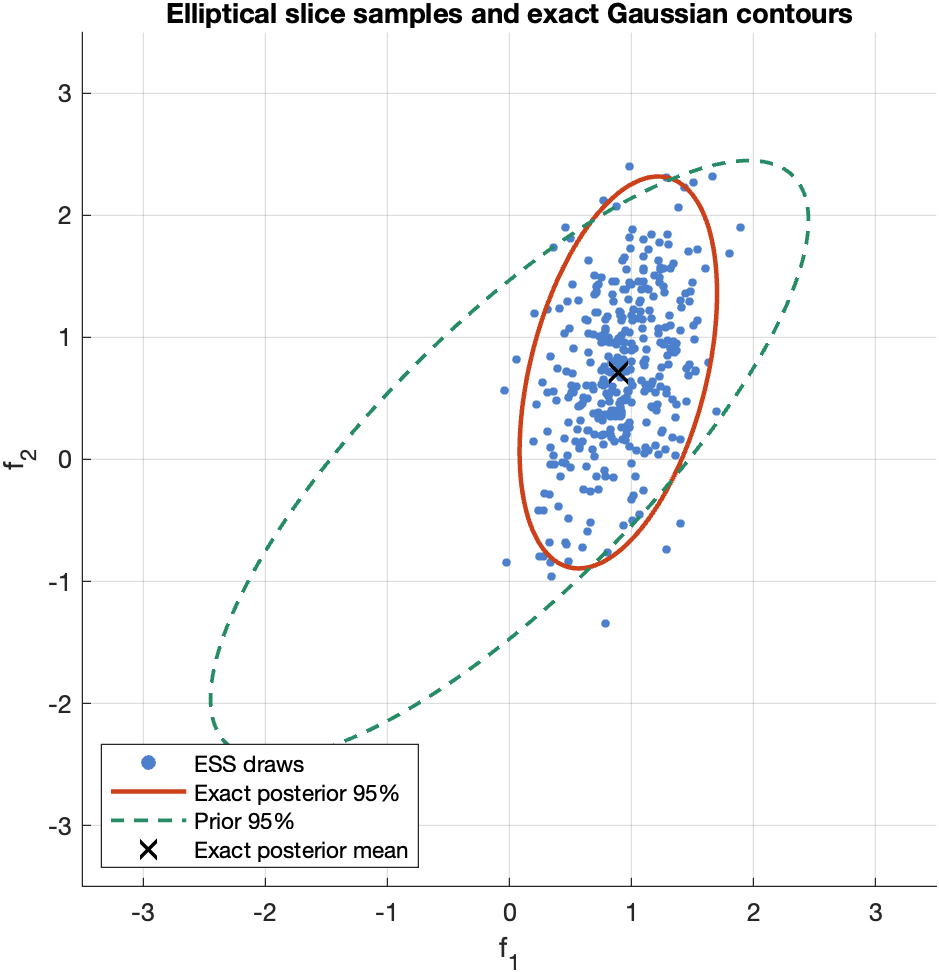
\includegraphics[width=0.88\textwidth,height=0.79\textheight,
                   keepaspectratio]{ess_demo.png}
\end{frame}

\begin{frame}{What the comparison checks}
  \begin{itemize}
    \setlength{\itemsep}{0.8em}
    \item The sample mean should be near \((0.891,\,0.713)^\top\).
    \item The sample cloud should follow the exact posterior contour,
          which is narrower than the prior in the \(f_1\) direction.
    \item This example has an exact posterior only because the likelihood
          is Gaussian. The same ESS code can use a different log-likelihood.
  \end{itemize}
  \vfill
  {\footnotesize Source: I. Murray, R. P. Adams and D. J. C. MacKay
  (2010), \emph{Elliptical slice sampling}, AISTATS, pp.\ 541--548.
  \url{https://proceedings.mlr.press/v9/murray10a.html}}
\end{frame}

\end{document}
